\documentclass [11pt, a4wide, twoside]{article}

\usepackage{times}
\usepackage{epsfig}
\usepackage{ifthen}
\usepackage{xspace}
\usepackage{fancyhdr}
\usepackage{hyperref}

% solution switch
\newboolean{showsolution}
\setboolean{showsolution}{false}


%layout
\topmargin      -5.0mm
\oddsidemargin  6.0mm
\evensidemargin -6.0mm
\textheight 215.5mm
\textwidth      160.0mm
\parindent        1.0em
\headsep          10.3mm
\headheight        12pt
\lineskip    1pt
\normallineskip     1pt

%header
\lhead{Programming Languages \\ 2021}

\rhead{Prof. O. Nierstrasz\\
Mohammadreza Hazhirpasand, Joel Niklaus}
\lfoot{page \thepage}
\rfoot{\today}
\cfoot{}

\renewcommand{\headrulewidth}{0.1pt}
\renewcommand{\footrulewidth}{0.1pt}

\renewcommand{\thesubsection}{\arabic{subsection}}

%enumeration
\newenvironment{myitemize}{%
     \begin{itemize}
     \setlength{\itemsep}{0cm}}
     {\end{itemize}}

\newenvironment{myenumerate}{%
     \begin{enumerate} \setlength{\itemsep}{0cm}}
     {\end{enumerate}}


%solution
\ifthenelse{\boolean{showsolution}}
   {  \newcommand{\solution}[1]{
   	\noindent\underline{\textbf{Answer:}}\\[2mm]
   	 \textsl{#1}
	 \vspace{10pt}
	 \normalsize
	}
  }
  {  \newcommand{\solution}[1]{} }

\newcounter{exnum}
\def\xexercise{\fontsize{12}{10}\fontseries{bx}\selectfont}
\def\xnormal{\fontseries{m}\fontshape{n}\selectfont}


\newcommand{\exercise}[1]{%
     {\addtocounter{exnum}{1}\vskip 0.8cm{\xexercise \noindent Exercise
\arabic{exnum} (#1)} \xnormal} \vskip 0.3cm} 
 \newcommand{\aufgabe}[1]{
     {\addtocounter{exnum}{1}\vskip 0.8cm{\xexercise \noindent Aufgabe
\arabic{exnum} (#1)} \xnormal} \vskip 0.3cm} 

\pagestyle{fancy}


% ===============ABBREVIATIONS==============================
\newcommand{\eg}{\emph{e.g.,}\xspace}
\newcommand{\ie}{\emph{i.e.,}\xspace}
\newcommand{\etc}{\emph{etc.}\xspace}


\begin{document}

% title
\section*{\ifthenelse{\boolean{showsolution}}{Solution\space{}}{}Serie 3 - Haskell}
% - - - - - - - - - - - - - - - - - - - - - - - - - - - - - - - - - - - - - - - - - - - - - - - - - - - - - - - - - - - - - - - - - - -
\subsection*{Exercise 1}

\begin{figure}[htb]
\begin{minipage}{.65\textwidth}
A \emph{triangular number} is the number of objects that can be arranged in a triangle as is shown in Fig. 1. This is how bowling pins, pool balls, or snooker balls are arranged. The figure shows the first six triangular numbers: 1, 3, 6, 10, 15, 21.

The \emph{tetrahedral number} represents the number of objects arranged in a pyramid (more precisely, a tetrahedron) built up from triangles as shown in the Figure.
\end{minipage}
\begin{minipage}[c]{.35\textwidth}
    \center{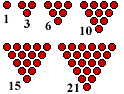
\includegraphics[width=3cm]{triang}\caption{Triangular numbers.\label{figure:triangularNumbers}}}
\end{minipage}
\end{figure}

\noindent The exercise:
\begin{itemize}
\item Write two functions to calculate the n-th triangular number, using classical recursion and tail recursion, respectively.
\item Write two functions to calculate the n-th tetrahedral number, using patterns and guards, respectively. \textbf{Hint:} use the function from the preceding exercise.
\end{itemize}

\solution{\texttt{factors :: Int -> [Int]}\\
since both \texttt{n} and \texttt{x} are arguments of the function \texttt{mod} which accepts only the \texttt{Int} arguments\\
\\
\texttt{isPerfect :: Int -> Bool}\\
since \texttt{n} is an argument of the function \texttt{factors} which accepts only the \texttt{Int} arguments,\\
and \texttt{== :: Eq a => a -> a -> Bool}\\
\\
Both functions are monomorphic.\\
\texttt{-----------------------------------------------------------------------}\\
\texttt{insert :: Int -> a -> [a] -> [a]}\\
since\\
\texttt{insert \_ n l = [n] => insert :: a->b->c->[b]}\\
\texttt{insert 0 n l = n:l => insert :: Int->b->[b]->[b]}\\
The \texttt{insert} function is polymorphic.

\texttt{mH (a, b, c) = c} \\

\texttt{mH :: (x, y, z) -> z}\\
mH is polymorphic since the three elements a, b, and c may be of any type. \\}

% - - - - - - - - - - - - - - - - - - - - - - - - - - - - - - - - - - - - - - - - - - - - - - - - - - - - - - - - - - - - - - - - - - -

\subsection*{Exercise 2\footnote{This exercise is an adaption of problem 6 from \url{http://projecteuler.net/}. You can find a ton of cool problems there.}}

The sum of the squares of the first ten natural numbers is,

$1^2 + 2^2 + ... + 10^2 = 385$

The square of the sum of the first ten natural numbers is,

$(1 + 2 + ... + 10)^2 = 55^2 = 3025$

Hence the difference between the sum of the squares of the first ten natural numbers and the square of the sum is $3025 - 385 = 2640.$

Write a Haskell program to find the difference between the sum of the squares of the first one hundred natural numbers and the square of the sum.

OPTIONAL: Implement the same solution in you favorite non functional language and discuss the differences.


\solution{and $\equiv$ $\lambda$~x y .~x y x \\
	\indent\indent // if the first argument is \texttt{False}, the function should return \texttt{False}, \ie the first argument; \\
	\indent\indent // if the first argument is \texttt{True}, the function should return the second argument\\
or $\equiv$ $\lambda$~x y .~x x y \\
	\indent\indent // if the first argument is \texttt{True}, the function should return \texttt{True}, \ie the first argument; \\
	\indent\indent // if the first argument is \texttt{False}, the function should return the second argument\\

\texttt{True and False = False}\\
\indent\indent ($\lambda$~x y.~x y x)($\lambda$~x y.~x)($\lambda$~x y.~y) = \\
\indent\indent ($\lambda$~x y.~x)($\lambda$~x y.~y)($\lambda$~x y.~x) = \\
\indent\indent ($\lambda$~x y.~y) $\equiv$ \texttt{False} \\

\texttt{True or False = True}\\
\indent\indent ($\lambda$~x y.~x x y)($\lambda$~x y.~x)($\lambda$~x y.~y) = \\
\indent\indent ($\lambda$~x y.~x)($\lambda$~x y.~x)($\lambda$~x y.~y) = \\
\indent\indent ($\lambda$~x y.~x) $\equiv$ \texttt{True} \\}
% - - - - - - - - - - - - - - - - - - - - - - - - - - - - - - - - - - - - - - - - - - - - - - - - - - - - - - - - - - - - - - - - - - -
\subsection*{Exercise 3}

In this exercise, you are going to implement a set of functions which operate on lists. Their semantics are given below.

\begin{enumerate}
\renewcommand{\theenumi}{\alph{enumi}}
\item Write a function \verb+insertNode+ which adds a new node to the list. The new node should be inserted before the first node with a higher value (we assume that all lists to contain numbers).
\item Write a function \verb+deleteNodes+ which deletes all nodes which satisfy a certain predicate \verb+p+.
\item Write a function \verb+removeDuplicates+ which removes duplicates to get a list with nodes having unique values.
\item Write a function \verb+sumNodes+ which calculates the sum of all nodes of the list.
\item Write a mapping function \verb+mapList+ which applies to each node of the list a given function \texttt{f}, e.g., the \verb+square+ function, and returns a list with the resulting values.
\item Write a function \verb+mergeLists+ which merges two sorted lists to produce one list which is also sorted.\label{lb}
\item Use the function from \ref{lb} to implement a sorting function \verb+sortList+ which sorts a list in ascending order. A \emph{Mergesort} would be adequate in this case.
\end{enumerate}


\noindent The idea is to write for each function unit tests. There is a testing framework called HUnit, very similar to JUnit. To implement and use test cases,  you have to import HUnit as a module in your source file like 
this:

\fontsize{8pt}{10pt}
\begin{verbatim}
import HUnit
...
tests = TestList [
  (TestCase (assertEqual "error message" [1,2,2,3] (insertNode 2 [1..3]))),
  (TestCase (assertEqual "error message" [2,4,6] (deleteNodes odd [1..6]))) ]
...
run = do runTestTT tests
\end{verbatim}
\fontsize{10pt}{12pt}

\noindent Now to run your tests, you can just call \texttt{run}.\\

\noindent \textbf{Hint:} work test-driven, i.e. first write appropriate tests, then code your functions until the tests are 
``green''.\\

\solution{\fontsize{8pt}{10pt}
\begin{verbatim}
% --------------------------------------------------
% Squares
% --------------------------------------------------
/inch {72 mul} def
/centersquare
  { newpath
    .5 .5 moveto
    -.5 .5 lineto
    -.5 -.5 lineto
    .5 -.5 lineto
   closepath
  } def

  2.5 inch 6 inch translate
  1 16 div setlinewidth
  1 1 5 
  { gsave
      .5 mul inch dup scale
      centersquare
      stroke
    grestore
  } for
showpage

% --------------------------------------------------
% Rotation
% --------------------------------------------------
/Times-Roman findfont
10 scalefont
setfont
300 500 translate
0 10 540 {              % go from 0 to 540 degrees in 10 degree steps
  gsave                 % keep rotations temporary
    dup rotate          % rotate by degrees on stack from 'for'
    8 div 0 moveto      % divide angle by 8 and use it to shift in x direction.
    (postscript) show
  grestore              % get back the unrotated state

} for                   % iterate over angles
showpage
\end{verbatim}}


% - - - - - - - - - - - - - - - - - - - - - - - - - - - - - - - - - - - - - - - - - - - - - - - - - - - - - - - - - - - - - - - - - - -

%\subsection*{Exercise 5}
%
%Define the following functions:
%
%\begin{myitemize}
%	\item Define a function \texttt{nondecreasing} that takes a list \texttt{xs} as parameter and returns \texttt{True} iff the elements of \texttt{xs} are in non-decreasing order.
%
%	\item Define a more general function \texttt{goodlist} that takes a list \texttt{xs} and a predicate \texttt{p} as parameters and returns \texttt{True} iff each adjacent pair of elements in \texttt{xs} satisfies \texttt{p}.
%	
%	\item Now use the function \texttt{goodlist} to define further functions:
%
%		\begin{myitemize}
%			\item A function \texttt{alternating} that takes a list of numbers \texttt{xs} as parameter and returns \texttt{True} iff the elements of \texttt{xs} alternate odd and even.
%
%			\item A function \texttt{partial} that takes a list of numbers \texttt{xs} as parameter and returns \texttt{True} iff each number \texttt{x} in \texttt{xs} is either a multiple or a factor of the number preceding \texttt{x}.
%		\end{myitemize}
%\end{myitemize}
%
%\solution{\vspace{-20pt}\noindent \input{exercise5.tex}}

\end{document}
